
The Fourier Volume Reconstruction (FVR) method described in sections \ref{Sec:VolumeRegistrationSection} and \ref{Sec:AFVRApproach} were designed to be independent of RGB-D information input and thus sensors. As long as greyscale data with a depth component, RGB data with a depth component or depth data on their own are input, the FVR method should be able to compute accurate relative dense 3D reconstructions and optionally relative camera pose data. This section details both RGB-D sensor input advantages and disadvantages as well as those for monocular video input. Input via a stereo setup is also discussed. However, since there is much research on stereo methods which often reach accuracy which approaches RGB-D sensors, more focus is given to depth sensor based input as well as monocular video input, which is the most difficult data to work with. \\

\subsubsection{Depth Sensor Based Reconstruction}

Depth sensor input is advantageous for several reasons. It is faster than both stereo and monocular methods, and has more robustness and reliability. In general, it is also more accurate than stereo methods, and in most cases is more accurate than monocular based methods. The major disadvantage in using such sensors has historically been one of accessibility. Thanks to systems such as the Microsoft Kinect and the Asus Xtion Pro Live camera being available to the general public at a low expense, this is changing. However, there is still a mass of legacy video data which does not have actively generated depth data provided, moreover there is still a wealth of content still being produced by simple RGB cameras. \\

Another drawback of this method is that of accuracy. The accuracy of both the Kinect and Asus Xtion Pro Live sensors is limited to the resolution of the device. To alleviate this, some sub-pixel resolution generating algorithms may be used. These methods can be used in an attempt to generate greater resolution for given depth data. Methods may work on frames in a standalone fashion, although additional data such as consecutive frames and multi-camera techniques may also be used. Both the Microsoft Kinect and Asus Xtion Live Pro have maximum resolutions of $640 \times 480$. Methods of depth generation based on stereo data input (as well as monocular input) are capable of generating dense depth information at resolutions only limited by the resolution of the cameras used. As of 2017, most cameras, even those found on mobile devices, can generate video data at resolutions of $1024 \times 1080$. \\

Another possible drawback in using RGB-D sensors is that certain materials reflect the infra-red light used by such active cameras to compute the depth information. These sensors are also known to produce noise depth data around the corners and edges of objects captured within the frame. Since most computer vision algorithms make use of such salient features such as edges and corners within the image data, this can lead to inaccurate 3D reconstructions, especially in cases where 2D feature matching is used with RANSAC to produce 3D camera pose information. These sensors are also limited to indoor environments, their infra-red sensor components are saturated in the sunlight, and therefore little to no useful depth data may be generated in full sunlight. This is a major drawback as much of the world is made up of complex outdoor environments, therefore this is an unfortunate restriction given the usefulness of such cameras in indoor environments and lower light environments. \\

Another major disadvantage is that these sensors cannot produce depth data over distances. This is to do with the range of the active infra-red projection component of these sensors. Because the projection cannot reach far distances, the infra-red sensor cannot detect depth. This is in contrast to stereo and monocular methods which are capable of distant depth estimates.  

RGB-D camera sensors are still a popular choice for 3D reconstruction frameworks as the depth data produced by these methods is faster and more reliable than other sensors and techniques. For scenes and environments which can be accurately scanned by such depth sensors (such as environments with low sunlight, short ranges as in office environments and scenes with few objects which reflect infra-red light), RGB-D cameras are typically the preferred choice. The RGB-D data used to test the FVR method comes from an Asus Xtion Pro LIVE sensor. This sensor produces a colour and depth image input pair, which is processed in order to generate 3D volume frames which are the required input to the FVR method. \\

The color and depth image pair are referred to by $f(u,v)$ and $g(u,v)$ where $f(u,v)$ refers to the color image and $g(u,v)$ refers to the depth image. The colour image data contains a red, green and blue component each between the range $[0,255]$. Depth information is processed within the range $[0,10000]$. In terms of resolution, $u$ ranges $[0..639]$ and $v$ ranges $[0..479]$ giving a resolution of $640 \times 480$. Examples of images generated by the Asus Xtion Pro LIVE sensor are shown in figures \ref{fig:COLEXAMPLE} and \ref{fig:DEPTHEXAMPLE}. Given depth value for a given coordinate $u,v$, $Z_{u,v}$ is equal to the raw depth data value $g(u,v)$. Given coordinate $u,v$ and depth value $Z_{u,v}$ obtained via image $g$, $f(u,v)$ is projected into 3D space using equation \ref{eqn:PC_PROJECTION} to obtain the a-axis coordinate $X_{u,v}$ and y-axis coordinate $Y_{u,v}$. For each pixel value where depth information may be accurately recovered, the 3D point $[X_{u,v}, Y_{u,v}, Z_{u,v}]^T$ may be recovered. \\

From equation \ref{eqn:PC_PROJECTION}, the $X_{u,v}$ and $Y_{u,v}$ values are first translated relative to the center of the screen and then multiplied by the depth and attenuated by the focal length parameter. This is a typical projection function. In the equation, $c_x$ and $c_y$ represent the point where the optical axis intersects the projection plane (which occurs right at the center of the image, $c_x = 319.5$, $c_y = 239.5$. Parameters $f_x$ and $f_y$ represent the focal length which is defined as $f_x$, $f_y = 525.0$. \\


\begin{equation} \label{eqn:PC_PROJECTION}
\begin{split}
X_{u,v} & = \frac{(u - c_x)Z_{u,v}}{f_x} \\
Y_{u,v} & = \frac{(v - c_y)Z_{u,v}}{f_y} \\
\end{split}
\end{equation}

The FVR method requires that the point cloud generated by 3D points $[X_{u,v}, Y_{u,v}, Z_{u,v}]^T$ and colour data $f(u,v)$ be quantized for integration within a 3D volume. The volumes sizes used for testing were of sizes $128^3$, $256^3$ and $384^3$. Primarily, sizes $256^3$ and $384^3$ were used. It is common to use sizes which are an exponent of 2 for various computational reasons. However, $512^3$ was too large for the GPU used for testing (an NVIDIA GeForce 840 M GPU) so the maximum size $384^3$ was used for testing. The 3D point clouds were scaled to fit the volume, then their coordinates were rounded and integrated into the volume prior to registration. An example of a colour and depth image pair as well as the corresponding projection into different volume sizes ($128^3$ and $256^3$) are shown in figure \ref{fig:PROJECTED_FRAME}.  \\

Once the data has been projected into a volume, it may be used as input into the technique described in section \ref{Sec:AFVRApproach}. The algorithm may then compute the registration matrix required to merge two frames, the matrix is accumulated and used to integrate each frame in succession. Upon registration and integration of each frame, the final output 3D reconstruction may be obtained. \\

\begin{figure}[!htb] 
        \centering
        \begin{subfigure}[b]{1.8in}
                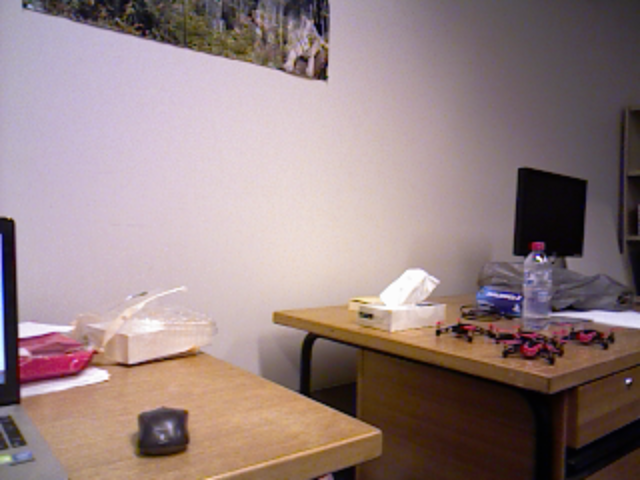
\includegraphics[width=1.7in]{images/ch2/colorF11}
                \caption{Color Image}
                \label{fig:COLEXAMPLE}
        \end{subfigure}%
        \begin{subfigure}[b]{1.8in}
                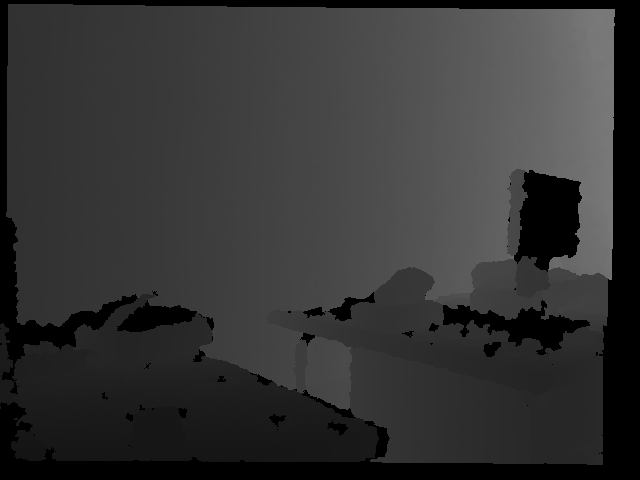
\includegraphics[width=1.7in]{images/ch2/depthF11}
                \caption{Depth Image}
                \label{fig:DEPTHEXAMPLE}
        \end{subfigure}
        
         \begin{subfigure}[b]{1.8in}
                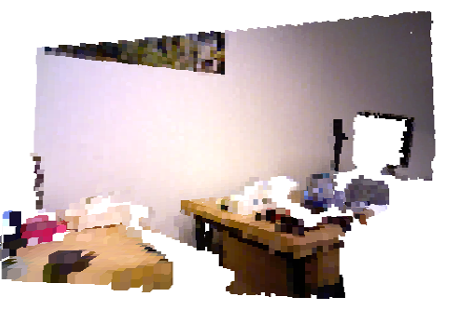
\includegraphics[width=1.8in]{images/ch2/volumeF11128}
                \caption{Projected Volume $128^3$}
                \label{fig:VOLUMEEXAMPLE128}
        \end{subfigure}%
         \begin{subfigure}[b]{1.8in}
                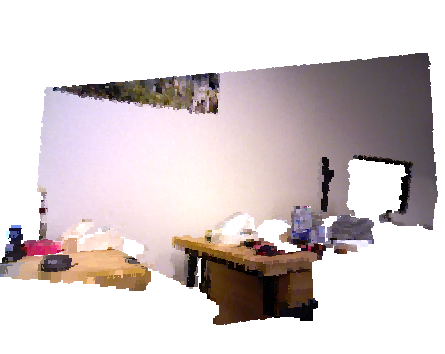
\includegraphics[width=1.8in]{images/ch2/volumeF11256}
                \caption{Projected Volume $256^3$}
                \label{fig:VOLUMEEXAMPLE384}
        \end{subfigure}%
       \caption{A Projected Frame.}
       \label{fig:PROJECTED_FRAME}
\end{figure}

\subsubsection{Stereo Camera Based Reconstruction}

As mentioned, the FVR method may take dense depth data from any type of input sensor, as long as dense 3D point clouds can be generated per frame or near per frame rates 3D reconstructions may be computed. Stereo methods do not produce depth data as fast or as reliably as compared to active sensors such as RGB-D cameras. However, they allow for higher resolution depth maps to be computed and may be used under environmental conditions where active cameras cannot work under. Additionally they are capable of generating depth data over larger ranges as compared to active camera approaches. \\

A major disadvantage is that depth maps are very noisy. Computing 3D reconstructions from depth data which have been produced via stereo methods is considerably more challenging. Still the noise is typically lower in comparison to monocular methods of depth estimation. In generating depth data using a stereo setup, the stereo camera pair must first be calibrated. The camera pair may be calibrated using software techniques to compute intrinsic camera parameters. Alternatively, the stereo data may be computed without first calibrating the stereo pair, resulting in less accurate depth data. Section \ref{StereoMethodsSection} described some of the available techniques in generating stereo data. \\

3D reconstruction from monocular view is considered a more difficult topic compared with 3D reconstruction generated from stereo views. For this reason, the use of monocular passive cameras was chosen to test the capabilities of the FVR method. The reason for choosing the more difficult topic of monocular 3D reconstructions is that stereo depth estimation is typically of higher quality. Therefore, if passable reconstructions could be computed based on this noisy monocular data, then 3D reconstructions based on stereo techniques (which produce significantly higher accuracy in terms of depth data generation) would be an easier task, relating more similarly to input obtained from RGB-D sensors. \\ 

\subsubsection{Monocular View Volume Reconstruction}

Generating dense depth information from monocular view is challenging. There are methods however, which take advantage of the properties of the Fundamental and Essential matrices to pre-calibrate consecutive frames. This allows stereo methods (see section \ref{StereoMethodsSection}) to be used to compute dense depth data per frame. These stereo methods are typically split into three categories: global, semi-global and local. Global methods are the most complex, and typically make use of some optimization method which optimizes the depth map's smoothness, disparity and contouring of edges jointly. Semi-global methods also optimize the depth map with respect to these requirements, however they are restricted to optimizing scan lines. This makes them much faster than the global optimization methods, whilst still providing better results than the local methods. Local methods are fast and ideal for real time applications, they make use of block matching to compute the disparity per pixel. \\

These methods all require frame by frame rectification. To do this, the fundamental matrix must be estimated accurately. The computation of the Fundamental matrix requires the use of feature matching and RANSAC which often are unable to accurately compute the Fundamental matrix. To generate dense depth data per frame, the use of optical flow based on 2D block matching was explored. By using 2D block matching, dense depth approximations were able to be computed whilst circumventing the use of the fundamental matrix and frame rectification. The depth maps computed are very noisy and inaccurate. The use of 2D spatial filtering as well as temporal filtering reduces such noise. \\

The spatial filtering technique used is basic Gaussian convolution. Temporal filtering was performed on a per pixel basis, where the output depth map is computed based on the previous depth map and the most recent depth map. Each depth map value is set to a value of $\delta \times prior-depth + (1-\delta) \times current-depth$. The best value for $\delta$ was judged based on qualitative analysis of experiment data sets. This method, although simpler and less accurate than other stereo methods, was used to test the FVR methods robustness to noisy and inaccurate 3D frame input. \\

 

The method presented here is named MVVR (Monocular View Volume Registration). The method takes in a set of monocular video frames, generates dense depth information from these frames before registering them geometrically and adding them into an output database. This output database is the dense 3D map. Pseudo code for this method is given in figure 1. Here, we go over the general algorithm. \\

The algorithm begins by reading in one frame at a time and placing frames in a queue structure. Once the queue has some pre-determined size, we pop the next frame and generate a disparity map from it and the current next frame. The threshold variable, skip is the amount of frames skipped when generating each disparity map. This is done so that there is sufficient change between frames to produce a reliable result without requiring subpixel accuracy. From the disparity maps a depth map is generated and added to a list called Input. Then for each depth map in Input and the next corresponding depth map after it, frames are projected and sampled into volumes for which translation, scaling and rotational information is computed using volume registration. This information allows us to merge depth data and generate a dense 3D map of the environment. \\

\begin{figure}
\begin{lstlisting}[language=c++,caption=Monocular View Volume Reconstruction,label=algorithm:MVVRAlgorithm,mathescape,basicstyle=\ttfamily]
let Input and q be Queues
let skip be an ℤ  [1,8]
let Pose be [0 0 0 ]T
let Camera be [0 0 0]T
let Cameras and Poses be Lists
let M be an Identity Matrix
Start
if no more frames then goto Part-2
f1 = readFrame()
q.add(f1)
if q.length < skip then goto Start
Input.add(BlockMatch(f1, queue.pop()))
goto Start
Part-2
PointCloud = project (Input[0])
Index = 0
Part-2-Start
if index == Input.length-1 then goto End
f1 = Input[index], f2 = Input[index+1]
points¬¬¬1 = project (f2), points2 = project (f1)
V1 = ResampleVolume (points¬¬¬1)
V2 = ResampleVolume (points2)
θ, φ, tx, ty, tz = VRθ,φ,tx,ty,tz (V1; V2)
M = M  TransformMatrix (θ, φ, tx, ty, tz)
Points1 = Transform (points1, M)
PointCloud = PointCloud  points1
Camera = M -1  Camera
Pose = M -1  Pose
Cameras.add(Camera)
 
Index++
goto Part-2-Start
End
\end{lstlisting}
\end{figure}

In order to generate depth maps, dense block matching is used to compute the camera motion induced disparity between frames. In our experiments we processed each framei with the 4th most recent frame, framei-4. For each image block in a frame, the displacement vector to the matching block in the next frame is computed. Using the concept of parallax we know that the magnitude of the displacement vector is an approximation to the actual depth at the corresponding location in the images. Due to noise the resulting displacement vectors can be very noisy. Figure 2 shows how noisy this estimated depth information can be compared with input from an RGB-D device. The noise can be largely eliminated using spatiotemporal filtering. \\



\begin{figure}[!htb]
\centering
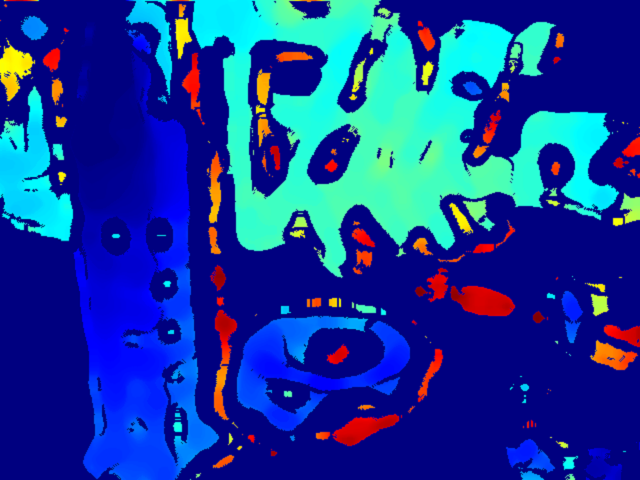
\includegraphics[width=6cm]{images/methodology/FVR/home_depth_frame_mono}
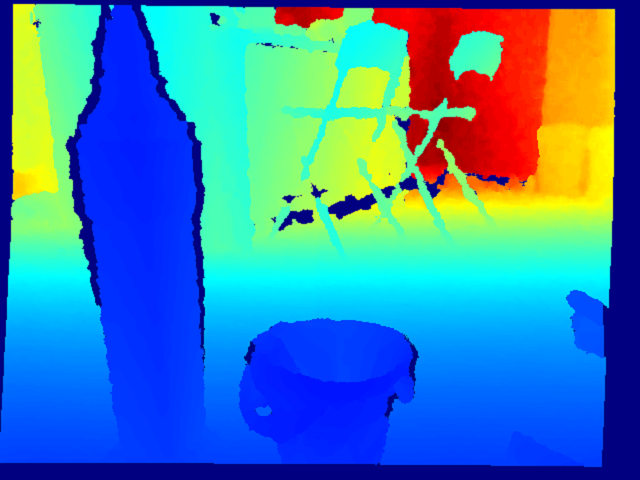
\includegraphics[width=6cm]{images/methodology/FVR/home_depth_frame}
\caption{Comparison between block matching estimated depth (left) and RGBD device depth (right).}
\label{fig:DepthGenerationExample}
\end{figure}
 


Figure 3 shows a functional block diagram of the volume registration method from [1]. The input data are two 3D volumes (Volume1 and Volume2), the output is the transformation matrix required to register them. The volumes are first Hanning windowed, reducing the effects of noise generated when transforming into the frequency domain. Next, a translation independent representation of each volume is obtained by taking the magnitude of their 3D FFTs. A log function is then applied to the resulting magnitude values; this improves estimation of scale and rotation [18]. \\

